\documentclass[a4paper,12pt]{article}

\usepackage{graphicx} % Required for inserting images
\usepackage{amsmath,amssymb,amsfonts}
\usepackage{subcaption}
% -----------------------
% Package Imports
% -----------------------

% Set page margins
\usepackage[a4paper, top=1in, bottom=0.8in, left=1.1in, right=0.8in]{geometry}

% Use Times New Roman font
\usepackage{times}

\usepackage{microtype}

\usepackage{array,booktabs,multirow,makecell}
\usepackage{bm}
\usepackage{siunitx}  % For proper unit handling


% Set page margins
\usepackage[a4paper, top=1in, bottom=0.8in, left=1.1in, right=0.8in]{geometry}


% Add page numbering
\pagestyle{plain}

% Enable graphics inclusion
\usepackage{graphicx}
\usepackage{float}
% Enable code listings
\usepackage{listings}
\usepackage{xcolor} % For customizing code colors
\setlength{\parindent}{0pt}
\usepackage{multirow}

\setlength{\parindent}{0pt}
\usepackage{titlesec} % To customize section font size
\titleformat{\section}
{\normalfont\fontsize{14}{16}\bfseries}{\thesection}{1em}{}

\titleformat{\subsection}
{\normalfont\fontsize{14}{16}\bfseries}{\thesubsection}{1em}{}

\begin{document}
	\section{Experiment No. 11}
	
	\section{Experiment Title}
	Observation of Speed-Torque Characteristic Curve of a 3-Phase Induction Motor.
	
	\section{Objective}
	
	The objectives of this lab are as follows:
	\begin{itemize}
		\item To observe the speed-torque characteristics of a 3-phase induction motor under varying load conditions
		\item To examine how slip and power factor change with increasing mechanical load
		\item To understand the practical implications of motor performance curves
	\end{itemize}
	
	\section*{Theory}
	
	Three-phase induction motors are widely used in industry due to their reliability and efficiency. When a 3-phase supply is given to the stator windings, a rotating magnetic field (RMF) is generated. This field induces current in the rotor, producing a secondary magnetic field that interacts with the RMF to generate torque.
	
	
		\begin{figure}[H]
		\centering
		\begin{subfigure}[t]{1\textwidth}
			\centering
			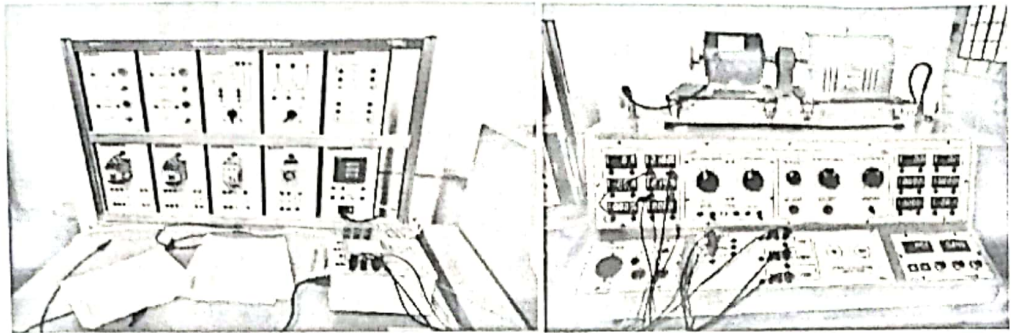
\includegraphics[width=0.9\textwidth]{Images/1}
			\caption{3-phase induction motor test setup}
			\vspace{0.1cm}
		\end{subfigure}
		
		\begin{subfigure}[t]{0.6\textwidth}
			\centering
			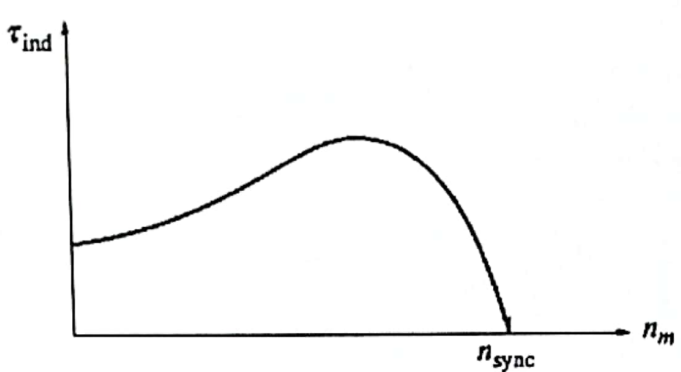
\includegraphics[width=1\textwidth]{Images/2}
			\caption{Speed-Torque Characteristic Curve of a 3-Phase Induction Motor}
		\end{subfigure}
	\end{figure}
	The synchronous speed ($N_s$) is given by:
	\[
	N_s = \frac{120f}{P}
	\]
	where $f$ is the supply frequency and $P$ is the number of poles.
	
	Slip ($S$), the difference between synchronous and rotor speed ($N_r$), is defined as:
	\[
	S = \frac{N_s - N_r}{N_s}
	\]
	
	Torque depends on slip, rotor resistance, and reactance. The torque-speed characteristic shows regions of operation from no load to maximum torque (pull-out torque). At low load, power factor is low due to dominant reactive power. As load increases, active power and power factor improve.
	
	\section{Circuit Diagram}
	\begin{figure}[H]
		\centering
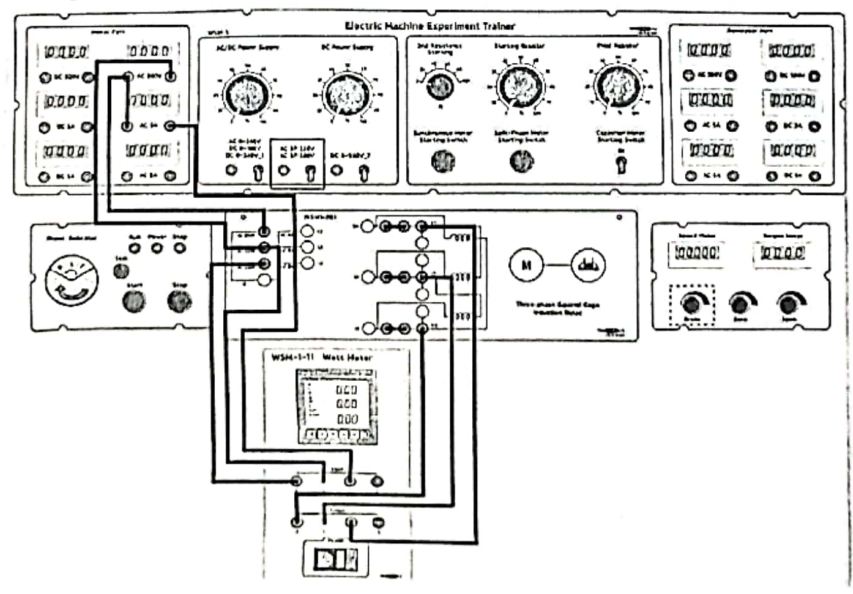
\includegraphics[width=0.7\linewidth]{Images/3}
		\caption{Circuit diagram for 3-phase induction motor test setup}
		\label{fig:circuit}
	\end{figure}
	
	\section{Required Apparatus}
	\begin{table}[H]
		\centering
		\caption{List of Required Equipment}
		\begin{tabular}{|c|p{5.5cm}|p{6cm}|}
			\hline
			\textbf{SN} & \textbf{Equipment} & \textbf{Specification} \\
			\hline
			1 & 3-Phase Induction Motor & Output: 360W, Voltage: 220V, Current: 2.2A, Speed: 1480 RPM \\
			\hline
			2 & Electric Machine Trainer & -- \\
			\hline
			3 & Dynamometer & Imax = 3A, Speedmax = 4000 RPM \\
			\hline
			4 & Star-Delta Switch & -- \\
			\hline
			5 & AC Multimeter & Vrmsmax = 500V, Imax = 5A \\
			\hline
			6 & Connecting Wires & -- \\
			\hline
		\end{tabular}
	\end{table}
	
	\section{Procedure}
	\begin{enumerate}
		\item Connect the motor to the dynamometer and measuring instruments as per the circuit diagram
		\item Start the motor with no load and record the initial speed, current, and power readings
		\item Gradually increase the mechanical load using the dynamometer
		\item At each load step, record:
		\begin{itemize}
			\item Motor speed (RPM)
			\item Torque (Nm)
			\item Current (A)
			\item Active power (W)
			\item Reactive power (VAR)
			\item Apparent power (VA)
			\item Power factor
		\end{itemize}
		\item Continue until the motor reaches near full-load conditions
		\item Plot the speed-torque characteristic curve
	\end{enumerate}
	
	\section{Result}
\begin{table}[H]
	\centering
	\caption{Experimental Data Table}
	\renewcommand{\arraystretch}{0.9}
	\scalebox{0.75}{
		\begin{tabular}{|c|c|c|c|c|c|c|}
			\hline
			\textbf{Speed (RPM)} & \textbf{Torque (Nm)} & \textbf{Current (A)} & \textbf{Active Power (W)} & \textbf{Reactive Power (VAR)} & \textbf{Apparent Power (VA)} & \textbf{Power Factor} \\
			\hline
			1497 & 0.001 & 1.972 & 181.1 & 754.2 & 774.1 & 0.23 \\ \hline
			1484 & 0.257 & 2.006 & 309.9 & 711.5 & 775.2 & 0.40 \\ \hline
			1479 & 0.315 & 2.021 & 360.0 & 708.0 & 792.5 & 0.45 \\ \hline
			1477 & 0.342 & 2.040 & 375.0 & 690.0 & 783.0 & 0.47 \\ \hline
			1474 & 0.379 & 2.062 & 390.0 & 692.0 & 792.0 & 0.49 \\ \hline
			1473 & 0.408 & 2.080 & 425.0 & 686.0 & 805.0 & 0.53 \\ \hline
			1469 & 0.443 & 2.120 & 475.0 & 687.0 & 833.0 & 0.57 \\ \hline
			1460 & 0.469 & 2.190 & 519.0 & 679.0 & 854.0 & 0.61 \\
			\hline
	\end{tabular}}
\end{table}


	
	\begin{figure}[H]
		\centering
	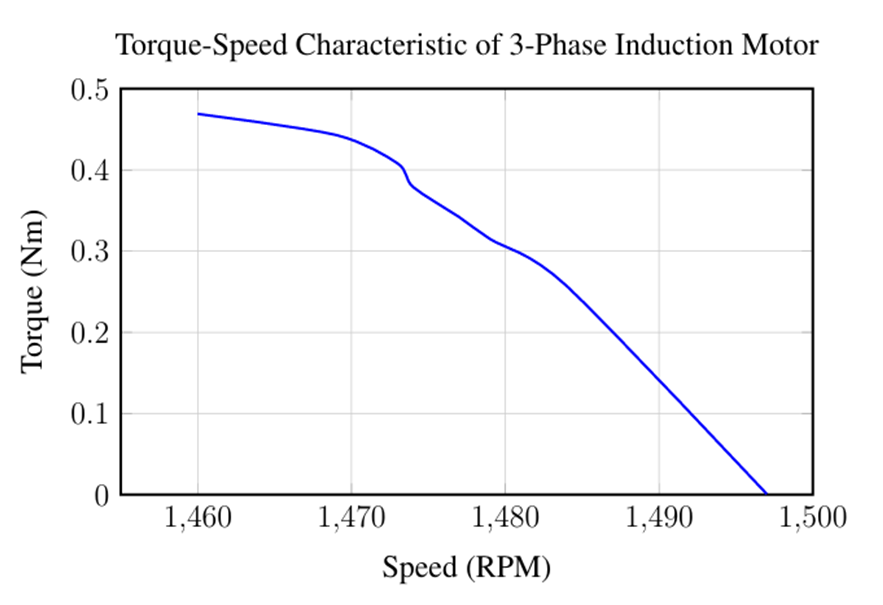
\includegraphics[width=0.68\linewidth]{Images/4}
		\caption{Speed-torque characteristic curve }
		\label{fig:results}
	\end{figure}
	
\section{Discussion}
The experimental results demonstrate key characteristics of the 3-phase induction motor. As mechanical load increases from 0.001 Nm to 0.469 Nm, the motor speed decreases slightly from 1497 RPM to 1460 RPM, showing the expected speed-torque relationship. This corresponds to increasing slip from 0.002 to 0.027. The power factor improves significantly from 0.23 (no-load) to 0.607 (full-load), indicating better energy utilization under load, while current increases moderately from 1.972A to 2.190A. These observations confirm theoretical predictions, with the speed-torque curve showing the characteristic downward slope and stable operation across the entire load range.

\section{Conclusion}
The experiment successfully characterized the induction motor's performance, showing: (1) minimal 2.5\% speed variation from no-load to full-load, (2) significant power factor improvement (0.23 to 0.607), and (3) stable operation matching theoretical predictions. These results validate the motor's design and suitability for industrial applications requiring consistent performance under varying loads.
	
	\section{Precautions}
	\begin{enumerate}
		\item Ensure all connections are secure before applying power
		\item Do not exceed the motor's rated current (2.2A) during testing
		\item Gradually increase the load to avoid sudden torque shocks
		\item Monitor temperature during prolonged operation
	\end{enumerate}
	
	\section{Reference}
	Stephen J. Chapman, \textit{Electric Machinery Fundamentals}.
\end{document}